\documentclass{beamer}

\usepackage[utf8]{inputenc}
\usepackage[french]{babel}
\usepackage[T1]{fontenc}
\usepackage{tikz}
\usetikzlibrary{shapes, arrows}

\usetheme{Montpellier}
%\usecolortheme{lily}

%STYLE
\tikzstyle{block} = [rectangle, draw, fill=blue!10,
	text width=5em, text centered, rounded corners, minimum width=100pt, minimum height=25pt]
\tikzstyle{cloud} = [draw, ellipse, fill=red!10, node distance=5cm, minimum height=2em]

\title{PSAR - Logika}
\author{Sandra \textsc{LADURANTI} et Bastien \textsc{RIGAULT}}
\date{2015-2016}
\begin{document}



	\begin{frame}
		
\includegraphics[width=0.20\textwidth]{logo}
		\titlepage
	\end{frame}
	
	\begin{frame}
		\frametitle{Sommaire}
		\tableofcontents
	\end{frame}
	
	\section{Architecture générale}
	\begin{frame}
	\begin{figure}
	\centering	
	
	
	\begin{tikzpicture}[node distance = 2cm, auto]
		%Place node		%Place node
		\node [block] (ui) {Interface graphique};
		\node [cloud, left of=ui] (uiAction) {Action utilisateur};
		\node [block, below of=ui] (ctrl) {Contrôleur};
		\node [cloud, left of=ctrl] (aig) {Aiguillage};
		\node [block, below of=ctrl] (mod) {Modèle};
		\node [cloud, left of=mod] (proc) {Traitement};
		
		%Draw edges
		\draw [->] (ui.-150) -- (ctrl.155);
		\draw [->] (ctrl.-130) -- (mod.130);
		\draw [->] (mod.50) -- (ctrl.-50);
		\draw [->] (ctrl.25) -- (ui.-30);
		
		\draw [->, dashed] (uiAction) -- (ui);
		\draw [->, dashed] (mod) -- (proc);
		\draw [->, dashed] (proc) -- (mod);
		
	\end{tikzpicture}
	\end{figure}
	\end{frame}
	
	\section{Exemple : Traitement d'une formule (1)}
	\begin{frame}
	\includegraphics[scale=0.4]{organisationProg}
	\end{frame}
	
	\section{Exemple : Traitement d'une formule (2)}
	\begin{frame}
	\centering
	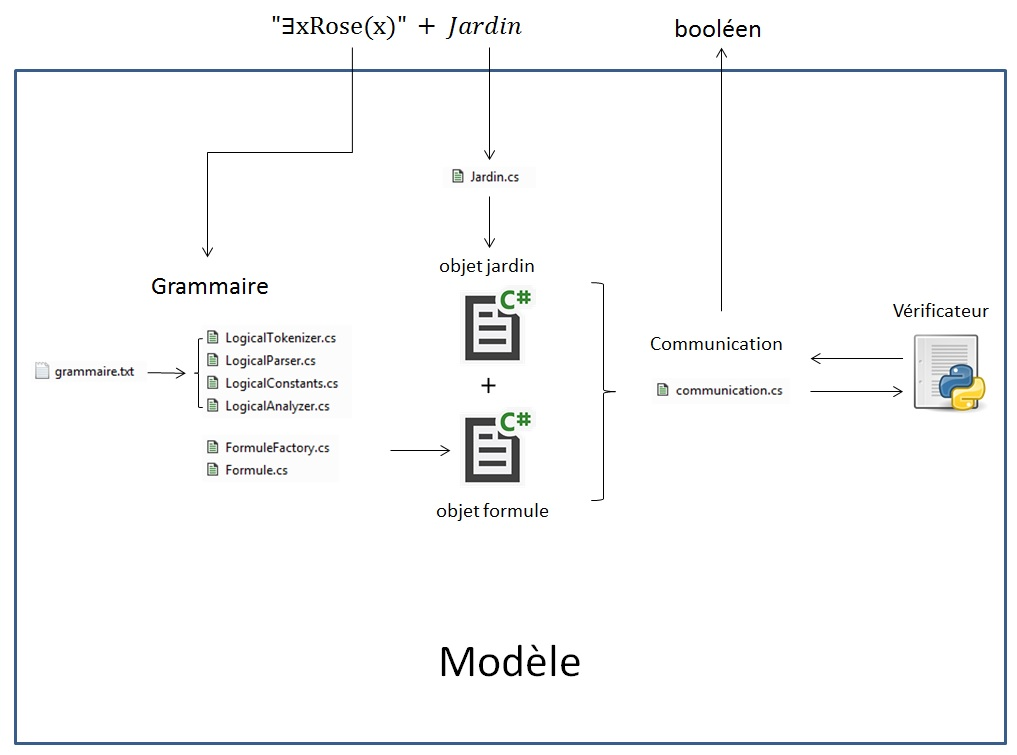
\includegraphics[scale=0.35]{communication}
	\end{frame}
	
	\section{Objectifs pour les prochaines semaines}
	\begin{frame}
	\begin{itemize}
		\setlength\itemsep{2em}
		\item Modélisation du plateau et des objets 3D
		\item Création du clavier visuel et du formulaire de saisie de formule
		\item Test approfondis du traitement de vérification de formule
	\end{itemize}
	\end{frame}
	
\end{document}